\documentclass[11pt,a4paper]{article}

% Version: injected by CI, or provide a fallback for local builds
\IfFileExists{version.tex}{\input{version.tex}}{\newcommand{\docversion}{dev}}

% ── Encoding & fonts ─────────────────────────────────────────────────────────
\usepackage{fontspec}
\setmainfont{Fira Sans}[
    BoldFont   = {Fira Sans Bold},
    ItalicFont = {Fira Sans Italic},
    BoldItalicFont = {Fira Sans Bold Italic},
]
\setsansfont{Fira Sans}
\setmonofont{FiraCode Nerd Font}[
    Scale = 0.85,
]
\renewcommand{\familydefault}{\sfdefault}
\usepackage{unicode-math}
\setmathfont{Fira Math}  % or remove this line and use \usepackage{newtxsf} if Fira Math is not installed

% ── Layout ───────────────────────────────────────────────────────────────────
\usepackage[margin=2.5cm]{geometry}
\usepackage{parskip}               % Paragraph spacing instead of indentation
\setlength{\parskip}{0.5\baselineskip}

% ── Bibliography ─────────────────────────────────────────────────────────────
\usepackage[backend=biber, style=numeric, sorting=none, date=short, urldate=short]{biblatex}
\addbibresource{references.bib}
% Force dd/mm/yyyy for all dates
\DeclareFieldFormat{urldate}{\mkbibparens{visited~#1}}
\renewcommand{\finentrypunct}{}

\AtEveryBibitem{%
  \iffieldundef{urldate}{}{\printfield{urldate}}%
}

% Override date formatting
\renewbibmacro*{urldate}{%
  \iffieldundef{urlyear}{}{%
    \printtext{\thefield{urlday}/\thefield{urlmonth}/\thefield{urlyear}}%
  }%
}

% removes In:
\renewbibmacro{in:}{%
  \ifboolexpr{%
     test {\ifentrytype{article}}%
     or
     test {\ifentrytype{inproceedings}}%
  }{}{\printtext{\bibstring{in}\intitlepunct}}%
}
% ── Colours ──────────────────────────────────────────────────────────────────
\usepackage[dvipsnames]{xcolor}
\definecolor{accent}{HTML}{3F51B5}
\definecolor{accentlight}{HTML}{C5CAE9}
\definecolor{accentdark}{HTML}{283593}
\definecolor{codebg}{HTML}{F5F5F5}
\definecolor{codefr}{HTML}{E0E0E0}
\definecolor{warnred}{HTML}{C62828}
\definecolor{tipblue}{HTML}{1565C0}
\definecolor{exgreen}{HTML}{2E7D32}

% ── Code listings ────────────────────────────────────────────────────────────
\usepackage{listings}

\lstdefinestyle{normal}{
    backgroundcolor=\color{codebg},
    basicstyle=\ttfamily\small,
    breakatwhitespace=false,
    breaklines=true,
    captionpos=b,
    commentstyle=\color{grey}\itshape,
    showstringspaces=false,
    frame=single,
    rulecolor=\color{codefr},
    framesep=5pt,
    xleftmargin=5pt,
    xrightmargin=5pt,
}

\lstdefinestyle{bashstyle}{
    backgroundcolor=\color{codebg},
    basicstyle=\ttfamily\small,
    breakatwhitespace=false,
    breaklines=true,
    captionpos=b,
    commentstyle=\color{green!50!black}\itshape,
    keywordstyle=\color{accent}\bfseries,
    stringstyle=\color{red!60!black},
    showstringspaces=false,
    frame=single,
    rulecolor=\color{codefr},
    framesep=5pt,
    xleftmargin=5pt,
    xrightmargin=5pt,
    language=bash,
    morekeywords={perf,docker,wget,tar,make,source,mv,git,grep,ls},
    literate={~}{\textasciitilde}{1}
}

\lstdefinestyle{diffstyle}{
    backgroundcolor=\color{yellow!5},
    basicstyle=\ttfamily\small,
    breaklines=true,
    frame=single,
    rulecolor=\color{codefr},
    framesep=5pt,
    xleftmargin=5pt,
    xrightmargin=5pt,
}

\lstdefinestyle{outputstyle}{
    backgroundcolor=\color{accentlight!15},
    basicstyle=\ttfamily\footnotesize,
    breaklines=true,
    frame=single,
    rulecolor=\color{codefr},
    framesep=5pt,
    xleftmargin=5pt,
    xrightmargin=5pt,
}

\lstset{style=normal}

% ── Boxes (tcolorbox) ───────────────────────────────────────────────────────
\usepackage[most]{tcolorbox}

\newtcolorbox{tipbox}[1][]{
    enhanced,
    colback=accent!4!white,
    colframe=accent,
    coltitle=white,
    fonttitle=\bfseries\sffamily,
    title={#1},
    sharp corners,
    boxrule=0pt,
    leftrule=3pt,
    top=6pt, bottom=6pt,
    left=8pt, right=8pt,
    attach boxed title to top left={yshift=-2mm, xshift=4mm},
    boxed title style={
        colback=accent,
        sharp corners,
        boxrule=0pt,
        top=2pt, bottom=2pt, left=6pt, right=6pt,
    },
}

\newtcolorbox{warnbox}[1][]{
    enhanced,
    colback=warnred!4!white,
    colframe=warnred,
    coltitle=white,
    fonttitle=\bfseries\sffamily,
    title={#1},
    sharp corners,
    boxrule=0pt,
    leftrule=3pt,
    top=6pt, bottom=6pt,
    left=8pt, right=8pt,
    attach boxed title to top left={yshift=-2mm, xshift=4mm},
    boxed title style={
        colback=warnred,
        sharp corners,
        boxrule=0pt,
        top=2pt, bottom=2pt, left=6pt, right=6pt,
    },
}

\newtcolorbox{exercisebox}[1][]{
    enhanced,
    colback=exgreen!4!white,
    colframe=exgreen,
    coltitle=white,
    fonttitle=\bfseries\sffamily,
    title={#1},
    sharp corners,
    boxrule=0pt,
    leftrule=3pt,
    top=6pt, bottom=6pt,
    left=8pt, right=8pt,
    attach boxed title to top left={yshift=-2mm, xshift=4mm},
    boxed title style={
        colback=exgreen,
        sharp corners,
        boxrule=0pt,
        top=2pt, bottom=2pt, left=6pt, right=6pt,
    },
}

% ── Tables, lists, math ─────────────────────────────────────────────────────
\usepackage{booktabs}
\usepackage{array}
\usepackage{enumitem}
\usepackage{amsmath}
\usepackage{multirow}

% ── Title styling ────────────────────────────────────────────────────────────
\makeatletter
\renewcommand{\maketitle}{%
    \begin{center}
        {\color{accent}\rule{\textwidth}{2pt}}\\[0.8em]
        {\LARGE\bfseries\color{accentdark} \@title \par}
        \vspace{0.6em}
        {\large\color{gray!70!black} \@author \par}
        \vspace{0.1em}
        {\small\color{gray!70!black} \@date \par}
        \vspace{0.1em}
        {\footnotesize\color{gray!70!black} Version:~\docversion \par}
        \vspace{0.1em}
        {\color{accent}\rule{\textwidth}{2pt}}
    \end{center}
    \vspace{1em}
}
\makeatother

% ── Section styling ──────────────────────────────────────────────────────────
\usepackage{titlesec}
\titleformat{\section}
    {\Large\bfseries\color{accent}}
    {\thesection}{0.8em}{}[\vspace{2pt}{\color{accentlight}\titlerule[1.5pt]}]
\titleformat{\subsection}
    {\large\bfseries\color{accentdark}}
    {\thesubsection}{0.6em}{}
\titleformat{\subsubsection}
    {\normalsize\bfseries\color{accentdark}}
    {\thesubsubsection}{0.5em}{}
\titleformat{\paragraph}
    {\normalsize\bfseries\color{accent}}
    {}
    {0em}
    {}
\titlespacing{\paragraph}{0pt}{0.8\baselineskip}{7pt}

% ── Section styling ──────────────────────────────────────────────────────────
\usepackage{xspace}
\newcommand{\perf}{\texttt{perf}\xspace}
\newcommand{\madgraph}{\mbox{MadGraph5\_aMC@NLO}\xspace}
\newcommand{\mgamc}{\mbox{MG5aMC}\xspace}
\newcommand{\cudacpp}{\mbox{CUDACPP}\xspace}

% ── Header / footer ──────────────────────────────────────────────────────────
\usepackage{fancyhdr}
\usepackage{lastpage}
\pagestyle{fancy}
\fancyhf{}
\renewcommand{\headrulewidth}{0pt}
\renewcommand{\headrule}{\hbox to\headwidth{\color{accent}\leaders\hrule height \headrulewidth\hfill}}
\fancyhead[L]{\small\color{accent}Profiling with \perf and Flamegraphs}
\fancyfoot[R]{\small\color{accent}\thepage/\pageref{LastPage}}
\fancyhead[R]{\footnotesize\color{gray!70!black}\docversion}

% ── Hyperlinks ───────────────────────────────────────────────────────────────
\usepackage[savepos]{zref} % for the form
\usepackage{hyperref}
\hypersetup{
    colorlinks=true,
    linkcolor=accentdark,
    urlcolor=accent,
    citecolor=accentdark,
    pdftitle={Profiling with perf and Flamegraphs},
    pdfauthor={Daniele Massaro},
}
\renewcommand{\DefaultOptionsofText}{
    bordercolor=black,
    backgroundcolor=white,
    bordersep=1pt
}



\title{Profiling with \perf and Flamegraphs\\[0.2em]
\large Hands-on exercises with \madgraph and \cudacpp}
\author{Daniele Massaro}
\date{16$^\textup{th}$ March 2026}

\begin{document}
\maketitle
\thispagestyle{empty}

\begin{abstract}
    In this exercise session, we will apply some of the profiling techniques discussed during the lectures to profile \madgraph with the \cudacpp for hardware-accelerated matrix element calculation instructions.
    We will use Linux \perf to collect various performance metrics, generate the flamegraphs, and understand the differences in between the original pure Fortran version of the code and the new version exploiting Single Instruction Multiple Data (SIMD) paradigm through CPU vector instructions.
    Finally, we will verify Amdahl's Law by observing the speedup of the code in the new architecture.
    For people having access to GPU hardware, it is possible to obtain the flamegraphs also in case of GPU offloading.
\end{abstract}

\tableofcontents
\newpage

% ============================================================================
\section{Background}
% ============================================================================

\madgraph (\mgamc) is a Monte Carlo event generator widely used in High Energy Physics, and by the main LHC experiments.
At its core, \mgamc is a meta-code: given a certain physics process, it is able to \emph{write} Fortran code that can be used to obtain \emph{physical events} describing the specified process.
This implies computing the corresponding scattering matrix elements, and performing the phase space integration, and event unweighting, tasks that are done by the generated program \textbf{MadEvent}.

The \textbf{\cudacpp} plugin, developed at CERN, enhances the capabilities of the code generator engine, allowing it to write C++ code that can exploit SIMD vector instructions on CPUs or be offloaded to GPUs, and which replaces the Fortran matrix element calculation.
The other parts of MadEvent (phase space, unweighting, \dots) stay unchanged.

The reason on why \cudacpp tackled the matrix element computation is clear when profiling the original Fortran code.

\begin{tipbox}[Trivia]
The name ``MadGraph'' comes from \emph{Madison}, Wisconsin, where the code was originally created.
It was born initially as a tool to automate Feynman diagram generation and matrix element calculation.
It became a fully-fledged event generator once the component MadEvent was developed.
\end{tipbox}

% ============================================================================
\section{Prerequisites}
% ============================================================================

Follow this decision tree to understand to which class you belong and take the necessary actions:

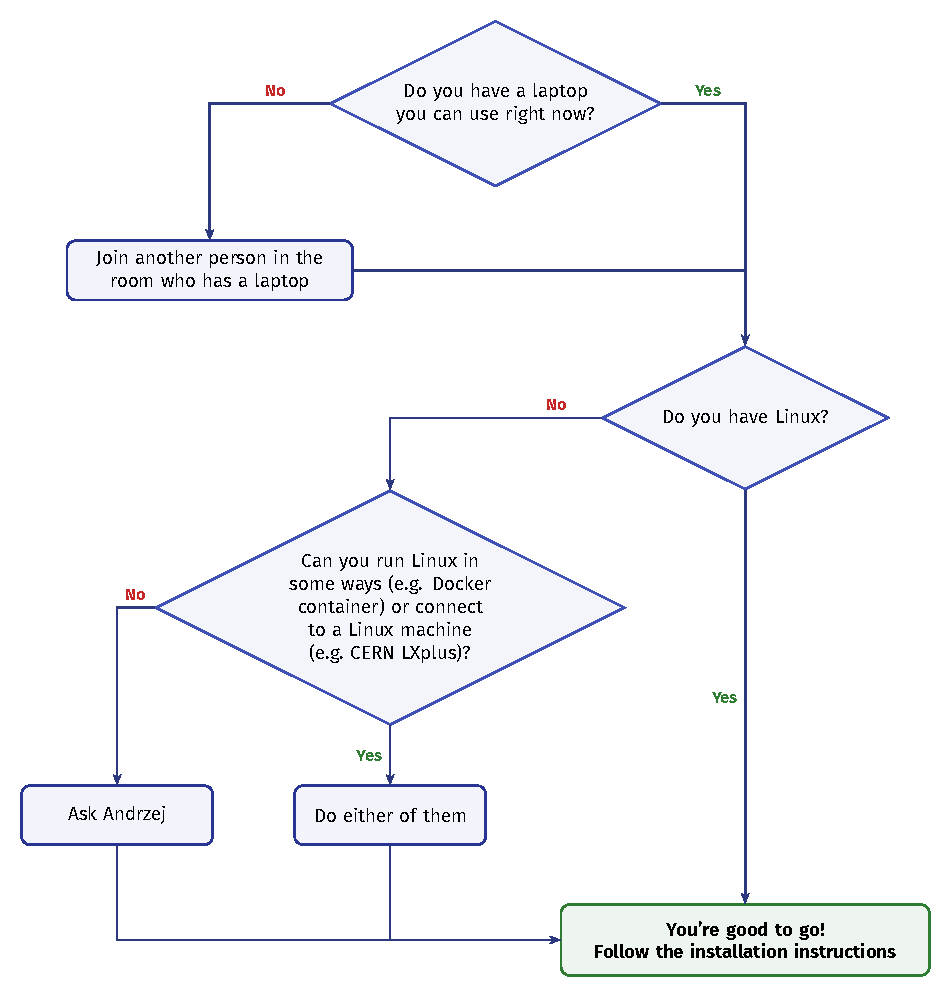
\includegraphics[width=\textwidth]{figures/choice-diagram}

\subsection{If you are using a/your Linux machine}

If you are using LXplus or a CERN-based machine with access to CVMFS, you can get the needed software by loading the stack \texttt{LCG\_108} for Alma Linux 9, built with GCC 14 with frame pointers enabled:
\begin{lstlisting}[style=bashstyle]
source /cvmfs/sft.cern.ch/lcg/views/LCG_108/x86_64-el9-gcc14fp-opt/setup.sh
\end{lstlisting}

Check that you fulfill the following:
\begin{itemize}[nosep]
    \item Python~3.9 or more, with the \texttt{six} package
    \item GCC and GFortran
    \item GNU Make
    \item \perf (if not available, install via \texttt{linux-tools-common}, \texttt{linux-tools-generic}, or\\ \texttt{linux-tools-\$(uname -r)} on Ubuntu/Debian)
    \item Perl (to generate FlameGraphs)
\end{itemize}

Before starting, check that \perf works:
\begin{lstlisting}[style=bashstyle]
perf stat ls
\end{lstlisting}

\subsection{If you want to use the Docker image}
First, verify you have Docker installed in your Linux distribution, see the \href{https://docs.docker.com/engine/install/}{official instructions}.

A Docker image is provided with MadGraph, the CUDACPP plugin, the FlameGraph tools, and \perf pre-installed.

\begin{lstlisting}
docker pull ghcr.io/qubitol/madgraph-profiling-exercises:latest
\end{lstlisting}

\begin{tipbox}[macOS / Apple Silicon users]
The Docker image works natively on Apple Silicon without x86 emulation.
CUDACPP supports ARM NEON through the \texttt{cppsse4} backend, so \textbf{Mac users using the Docker image should use \texttt{cppsse4} as the backend when running MadGraph}.
\end{tipbox}

\subsubsection{Running the container}

The tool \perf accesses hardware performance counters through the host kernel, so the container must run with elevated privileges:
There are two options.

\paragraph{Option A: \texttt{--privileged} (simplest)}

\begin{lstlisting}
docker run -it --rm \
  --privileged \
  --pid=host \
  ghcr.io/qubitol/madgraph-profiling-exercises:latest
\end{lstlisting}

\paragraph{Option B: fine-grained capabilities (more restrictive)}

\begin{lstlisting}
docker run -it --rm \
  --cap-add SYS_ADMIN \
  --cap-add SYS_PTRACE \
  --security-opt seccomp=unconfined \
  --pid=host \
  ghcr.io/qubitol/madgraph-profiling-exercises:latest
\end{lstlisting}

% https://medium.com/@geekidea_81313/running-perf-in-docker-kubernetes-7eb878afcd42
\begin{warnbox}[Host-side prerequisites]
The \textbf{host machine} must allow unprivileged access to performance counters.
You can check that the following options have been set (before running the container): \texttt{sysctl kernel.perf\_event\_paranoid} should return \texttt{-1};
If not, you can try to set it
\begin{lstlisting}
sudo sysctl kernel.perf_event_paranoid=-1
\end{lstlisting}
\end{warnbox}

\subsubsection{What is inside the container}

\begin{center}
\begin{tabular}{ll}
\toprule
\textbf{Component} & \textbf{Location} \\
\midrule
MadGraph5 & \texttt{\textasciitilde/MadGraph5/} \\
CUDACPP plugin & \texttt{\textasciitilde/MadGraph5/PLUGIN/} \\
FlameGraph scripts & \texttt{/opt/FlameGraph/} (also in \texttt{PATH}) \\
\texttt{perf} & \texttt{/usr/bin/perf} \\
\bottomrule
\end{tabular}
\end{center}

\subsubsection{Verifying the setup}

Once inside the container, run the provided check script:

\begin{lstlisting}
./check_perf.sh
\end{lstlisting}

This tests that \texttt{perf stat} and \texttt{perf record} work correctly.
If any test fails, verify that you started the container with the correct privileges and that the host-side \texttt{sysctl} settings are in place.

\subsubsection{Extracting files from the container}

Flamegraph SVGs and other outputs can be copied to the host while the container is running:

\begin{lstlisting}
# From the host:
docker cp <container_id>:/home/user/path/to/flamegraph.svg .
\end{lstlisting}

Alternatively, mount a host directory as a volume when starting the container:

\begin{lstlisting}
docker run -it --rm --privileged --pid=host \
  -v $(pwd)/output:/home/user/output \
  ghcr.io/qubitol/madgraph-profiling-exercises:latest
\end{lstlisting}

Files placed in \texttt{\textasciitilde/output/} inside the container will then appear in the \texttt{output/} directory on the host.

% ============================================================================
\section{Exercise 1: Installation}
\label{sec:installation}
% ============================================================================

\subsection{Install MadGraph}

\begin{lstlisting}[style=bashstyle]
wget https://github.com/mg5amcnlo/mg5amcnlo/archive/refs/tags/v3.6.6.tar.gz
tar xzf v3.6.6.tar.gz
mv mg5amcnlo-3.6.6 MadGraph5
cd MadGraph5
\end{lstlisting}

Every subsequent command assumes you are inside the \texttt{MadGraph5} directory.
The code can be run by running the following

\begin{lstlisting}[style=bashstyle]
./bin/mg5_aMC
\end{lstlisting}


\subsection{Install the CUDACPP plugin}

The CUDACPP plugin provides the hardware-accelerated matrix element implementations.
Install it through the MadGraph CLI:

\begin{lstlisting}[style=bashstyle]
./bin/mg5_aMC <<EOF
install cudacpp
EOF
\end{lstlisting}

Or, more simply, open MadGraph, run \texttt{install cudacpp}, and then wait for it to finish.

The plugin will be placed in the \texttt{PLUGIN/} directory.

\subsection{Install the FlameGraph scripts}

We will use Brendan Gregg's FlameGraph tools to convert \perf data into Flamegraphs:

\begin{lstlisting}[style=bashstyle]
cd ..
git clone https://github.com/brendangregg/FlameGraph.git
export FLAMEGRAPH_DIR=$(pwd)/FlameGraph
cd MadGraph5
\end{lstlisting}

\subsection{Check your machine's vectorisation support}
\label{sec:check_simd}

Before choosing a CUDACPP backend to run, check the compiler flags by reading \texttt{/proc/cpuinfo}, or by running `lscpu`, you should find that at least \texttt{sse4\_2} and \texttt{avx}/\texttt{avx2}.

\begin{lstlisting}[style=bashstyle]
grep -o -E 'sse4_2|avx2|avx512f|avx512bw|avx512vl' /proc/cpuinfo
\end{lstlisting}

The output tells you which backends you can use:
\begin{itemize}[nosep]
    \item \texttt{sse4\_2} $\to$ backend \texttt{cppsse4} (128-bit, 2 doubles per instruction)
    \item \texttt{avx2} $\to$ backend \texttt{cppavx2} (256-bit, 4 doubles per instruction)
    \item \texttt{avx512f} + \texttt{avx512bw} + \texttt{avx512vl} $\to$ backends \texttt{cpp512y} or \texttt{cpp512z} (8 doubles per instruction)
\end{itemize}

\begin{exercisebox}[Exercise 1]
Install MadGraph, the CUDACPP plugin, and the FlameGraph tools.
Verify that \perf works.
Check which SIMD instruction sets your machine supports and decide which backend you will use in the following exercises.
Specify here the backend: \TextField[name=backend, width=2.5cm]{}
\end{exercisebox}

% ============================================================================
\section{Exercise 2: Generate a process and test the setup}
\label{sec:generate}
% ============================================================================

\subsection{Generate the process}

We will use the process $gg \to t\bar{t}gg$ (gluon annihilation into a top--antitop pair with two additional gluons) as our benchmark.
This process has many Feynman diagrams, making the matrix element calculation computationally expensive and therefore an interesting profiling target.

To generate this process, we will use the MadGraph command-line interface.
Start MadGraph
\begin{lstlisting}[style=bashstyle]
./bin/mg5_aMC
\end{lstlisting}

And run the following commands, one at a time:
\begin{lstlisting}
generate g g > t t~ g g
output madevent_simd MY_PROCESS
\end{lstlisting}

The first command will generate all the possible feynman diagrams, while the second one will \emph{write the code} needed to perform the event generation.
You will find out a new folder named \texttt{MY\_PROCESS} can be found in the current working directory.

\begin{tipbox}[Output modes]
The output mode determines which backends are available:
\begin{itemize}[nosep]
    \item \texttt{madevent\_simd}: enables CPU backends (\texttt{cppnone}, \texttt{cppsse4}, \texttt{cppavx2}, \texttt{cpp512y}, \texttt{cpp512z})
    \item \texttt{madevent\_gpu}: enables GPU backends (CUDA, HIP)
\end{itemize}
\end{tipbox}

\subsection{Run a first test}

Now we will run the generated code, using the \texttt{launch} command.
Restart MadGraph if you closed it, and run the following commands (replace \texttt{cppavx2} with the appropriate backend for your machine, see~\S~\ref{sec:check_simd}):

\begin{lstlisting}
launch MY_PROCESS
done
set cudacpp_backend cppavx2
set nevents 10000
\end{lstlisting}

The \texttt{done} command in the middle serves for the purpose of skipping one of the prompts.
Indeed, the \texttt{set} command can be used only in the second prompt, when the program is asking to modify \texttt{param\_card.dat} or \texttt{run\_card.dat}.

If this completes without errors and produces a cross-section result, your setup is working.

\subsection{Locate the \texttt{madevent} executable}

MadGraph creates one \texttt{madevent} executable per subprocess.
The various subprocesses are contained in the \texttt{SubProcesses} directory, in this case we have only one single subprocess directory (\texttt{P1\_gg\_ttxgg}):

\begin{lstlisting}[style=bashstyle]
cd MY_PROCESS/SubProcesses/P1_gg_ttxgg/
ls -la madevent
\end{lstlisting}

The \texttt{madevent} file is a symlink to the actual compiled binary (e.g.\ \texttt{madevent\_cpp} for the vectorised backend, and \texttt{madevent\_cuda} or \texttt{madevent\_hip} for the GPU backend).
The first launch also creates subdirectories \texttt{G1/}, \texttt{G2/}, \ldots, that represent the various \emph{integration channels of the phase space}.
The thing you need to know is that each one of them contains a text file, named \texttt{input\_app.txt}, with the parameters for that specific phase-space parametrisation.

When using \texttt{launch}, MadGraph orchestrate the run of the executable \texttt{madevent} on the different parametrisations determined by the \texttt{G*/} folders for a certain subprocess.
This means \texttt{madevent} represents the \emph{smallest} component of the full computation.
It is the script that it is worth profiling.

Test running \texttt{madevent} directly, it requires standard input that can be passed through the \texttt{input\_app.txt} file contained in a certain \texttt{G*/} folder (pick \texttt{G1/} for example):
\begin{lstlisting}[style=bashstyle]
./madevent < G1/input_app.txt
\end{lstlisting}

The code is instrumented with a timer, and at the end of this execution will show the total time spent in the computation of the Fortran overhead, of the matrix element, and the total time.

\begin{exercisebox}[Exercise 2]
Generate the $gg \to t\bar{t}gg$ process, launch it once to verify the setup, and then run the \texttt{madevent} executable directly from the \texttt{SubProcesses/P1\_gg\_ttxgg} directory.
\end{exercisebox}

% ============================================================================
\section{Exercise 3: Prepare for profiling}
\label{sec:prepare}
% ============================================================================

\subsection{Add debug symbols and frame pointers}

By default, the MadGraph build system does not provide debug symbols, nor frame pointers.
Frame pointers are very useful when using \perf to build a proper call stack, with the resulting flamegraphs showing less broken stacks or missing frames.

We need to modify two files.

\subsubsection{Fortran compilation flags}

Edit \texttt{Source/make\_opts} (from the root of \texttt{MY\_PROCESS}) and change the \texttt{GLOBAL\_FLAG} line:

\begin{lstlisting}[style=diffstyle]
# Original:
GLOBAL_FLAG=-O

# Change to:
GLOBAL_FLAG=-O2 -g -fno-omit-frame-pointer
\end{lstlisting}

This affects all Fortran code (MadEvent framework, matrix elements in the Fortran version).

\subsubsection{C++ and CUDA compilation flags}

Edit \texttt{SubProcesses/P1\_gg\_ttxgg/cudacpp.mk} and modify the following lines.

Change \texttt{CXXFLAGS}:
\begin{lstlisting}[style=diffstyle]
# Original:
CXXFLAGS = $(OPTFLAGS) -std=c++17 -Wall -Wshadow -Wextra

# Change to:
CXXFLAGS = $(OPTFLAGS) -std=c++17 -Wall -Wshadow -Wextra -O2 -g -fno-omit-frame-pointer
\end{lstlisting}

Change \texttt{OPTFLAGS}:
\begin{lstlisting}[style=diffstyle]
# Original:
OPTFLAGS = -O3

# Change to:
OPTFLAGS = -O2 -g -fno-omit-frame-pointer
\end{lstlisting}

\begin{warnbox}[AMD GPU users]
In case you are doing these exercises on an AMD GPU, there is an additional override of \texttt{OPTFLAGS} that should be updated:
\begin{lstlisting}[style=diffstyle]
# Original:
override OPTFLAGS = -O2

# Change to:
override OPTFLAGS = -O2 -g -fno-omit-frame-pointer
\end{lstlisting}
\end{warnbox}

\begin{tipbox}[Are these flags passed also to the GPU builds?]
In case of GPU builds, the main compiler, let's take \texttt{nvcc} (NVIDIA CUDA Compiler), does not support \texttt{-g -fno-omit-frame-pointer} flags (they are GCC flags).
However, we may want to properly profile and show on a flamegraph the functions of the C++ files that are built with \texttt{nvcc} but that do not imply any GPU offloading.
To do this, we can pass the \texttt{-g -fno-omit-frame-pointer} flags to the underlying compiler \texttt{g++}, used by \texttt{nvcc}, via \texttt{nvcc}'s \texttt{-Xcompiler} flags.
This is done automatically already during build if the variable \texttt{OPTFLAGS} is correctly updated with those flags (as described above).
The \texttt{OPTFLAGS} variable is used in the \texttt{nvcc} invocation.
\end{tipbox}

\subsection{Rebuild}

Clean and rebuild everything.
From the \texttt{SubProcesses/P1\_gg\_ttxgg/} directory:

\begin{lstlisting}[style=bashstyle]
make cleanall
make madevent_cpp_link       # build the C++ vectorised version
make madevent_fortran_link   # build also the Fortran-only version
\end{lstlisting}

This recipe \texttt{madevent\_*\_link} is present in the makefile to build at once all the files available in the different folders.

\subsection{Increase the number of events}

Profiling with a sampling profiler requires collecting enough samples to build statistically meaningful stack traces.
At low sampling frequency, e.g. 97\,Hz, a 1-second run yields only $\approx$97 samples, which may be too few for a meaningful flamegraph.
We ideally need to collect thousands of samples.

Edit \texttt{G1/input\_app.txt} and increase the number of events to at least \textbf{100\,000} for CPU runs (the first integer in the first line), and \textbf{1\,000\,000} for GPU runs (in case you are trying these exercises on the GPU).
The file would look like this (mind, also the two integer numbers next to the first integer changed as well):

\begin{lstlisting}[style=outputstyle]
100000 1 1 !Number of events and max and min iterations
0.1        !Accuracy
2          !Grid Adjustment 0=none, 2=adjust
1          !Suppress Amplitude 1=yes
0          !Helicity Sum/event 0=exact
1
\end{lstlisting}

\begin{exercisebox}[Exercise 3]
Modify the compilation flags as described, rebuild both the Fortran and vectorised versions of \texttt{madevent}, and increase the event count.
Verify that both binaries run correctly and do not finish instantly.
\end{exercisebox}

% ============================================================================
\section{Exercise 4: Flamegraphs}
\label{sec:flamegraphs}
% ============================================================================

\subsection{A brief reminder on flamegraphs}

Flamegraphs are a visualisation of profiling data invented by Brendan Gregg.
Each horizontal bar represents a function in the call stack.
The \textbf{y-axis} is the stack depth (with entry point at the bottom, and \emph{leaf} functions at the top).
The \textbf{x-axis} is sorted alphabetically to merge identical stacks; the \textbf{width} of each bar is proportional to the number of samples in which that function appeared.
Wider bars mean the function was on-CPU more often.

The workflow to produce a flamegraph is:
\begin{enumerate}[nosep]
    \item \textbf{record}: use \texttt{perf record} to collect stack samples;
    \item \textbf{collapse}: convert the raw stack traces into a folded format;
    \item \textbf{render}: generate an interactive SVG \emph{picture}.
\end{enumerate}

\subsection{Profile the Fortran baseline}
\label{sec:profile_fortran}

From the subprocess directory (\texttt{SubProcesses/P1\_gg\_ttxgg/}):

\paragraph{Record}

\begin{lstlisting}[style=bashstyle]
perf record --call-graph=fp,1024 -F 97  -- ./madevent_fortran < G1/input_app.txt
\end{lstlisting}

\begin{tipbox}[What does \texttt{--call-graph=fp,1024} do?]
This option tells \perf to use frame pointers (\texttt{fp}) to rebuild the stack of functions.
The numeric parameter after the comma is the maximum stack depth.
For this example, setting it to 1024 seems to be a good number.
\end{tipbox}

\paragraph{Collapse}

\begin{lstlisting}[style=bashstyle]
perf script | $FLAMEGRAPH_DIR/stackcollapse-perf.pl > fortran.folded
\end{lstlisting}

\paragraph{Render}

\begin{lstlisting}[style=bashstyle]
$FLAMEGRAPH_DIR/flamegraph.pl fortran.folded > flamegraph_fortran.svg
\end{lstlisting}

\begin{tipbox}[Why 97\,Hz and not 99 or 100?]
We use a prime number for the sampling frequency to avoid aliasing with periodic patterns in the code.
If the code has a loop that takes exactly 10\,ms per iteration, and you sample at 100\,Hz, every sample lands at the same point in the loop, and you don't want that, since it would introduce a bias in the profiling results.
Prime frequencies avoid these synchronisation issues.
\end{tipbox}

Open \texttt{flamegraph\_fortran.svg} in a web browser.
The SVG is interactive: practice hovering over bars to see function names and sample percentages, click to zoom into a subtree, or search to highlight functions matching your search pattern (you can even use regular expressions).

\begin{exercisebox}[Exercise 4a]
Generate the flamegraph for the Fortran baseline.
Identify the function that has been sampled the most, and note down its name, this is the current \emph{bottleneck}, and it will be the function that is going to be hardware-accelerated.
Write here the function name \TextField[name=fortran_bottleneck, width=4cm]{}.
Hover over it and note the percentage of total samples it accounts for, and write down this number as well: \TextField[name=fortran_bottleneck_percentage, width=1.5cm]{}\%.
From the standard output, you can also find the total wall-time, note it here as $T_\textup{Fortran} =$ \TextField[name=time_fortran, width=1.5cm]{} s.
\end{exercisebox}

\subsection{Profile the vectorised version}
\label{sec:profile_cpp}

Now profile the vectorised C++ version (replace \texttt{madevent\_cpp} with the appropriate binary name):

\begin{lstlisting}[style=bashstyle]
perf record --call-graph=fp,1024 -F 97 -- ./madevent_cpp < G1/input_app.txt
perf script | $FLAMEGRAPH_DIR/stackcollapse-perf.pl > cpp.folded
$FLAMEGRAPH_DIR/flamegraph.pl cpp.folded > flamegraph_cpp.svg
\end{lstlisting}

\begin{exercisebox}[Exercise 4b]
Generate the flamegraph for the vectorised version.
Compare it visually with the Fortran flamegraph:
\begin{itemize}[nosep]
    \item What happened to the function that in the Fortran case was sampled the most?
    \item Which functions are now proportionally more visible?
\end{itemize}
Also in this case, note down the percentage of total samples that function now accounts for: \TextField[name=cpp_bottleneck_percentage, width=1.5cm]{}\%.
Write also the total wall-time, $T_\textup{SIMD} =$ \TextField[name=time_cpp, width=1.5cm]{} s.

\vspace{3mm}

\TextField[name=exercise_4b_notes, height=3cm, width=\linewidth, multiline, value={...notes...}]{}
\end{exercisebox}

\subsection{Walking the stack: DWARF-based unwinding}

An alternative stack-walking method, called \emph{DWARF} is available.
It uses debug unwind tables instead of frame pointers:
\begin{lstlisting}[style=bashstyle]
perf record --call-graph=dwarf -F 97 -- ./madevent_fortran < G1/input_app.txt
\end{lstlisting}
This works even without frame pointers but produces larger \texttt{perf.data} files.

% ============================================================================
\section{Exercise 5: Amdahl's law verification}
\label{sec:amdahl}
% ============================================================================

Amdahl's law predicts the maximum overall speedup when only a fraction of the workload is accelerated:

\begin{equation}
    S_\textup{Amdahl} = \frac{1}{(1 - p) + \dfrac{p}{n}}
    \label{eq:amdahl}
\end{equation}

where $p$ is the fraction of runtime that can be parallelised and $n$ is the \emph{number of processors} you are parallelising over.

\subsection{Extract the data from the flamegraphs}

From the wall-clock times of both runs, it is possible to compute:
\begin{itemize}[nosep]
    \item $T_{\text{Fortran}} =$ \TextField[name=time_fortran_summary, width=1.5cm]{} s: total time for the Fortran run
    \item $T_{\text{SIMD}} =$ \TextField[name=time_cpp_summary, width=1.5cm]{} s: total time for the vectorised run
    \item $S_{\text{observed}} = T_{\text{Fortran}} \,/\, T_{\text{SIMD}} =$ \TextField[name=speedup, width=1.5cm]{}: the observed overall speedup
\end{itemize}

Additionally, from the Fortran flamegraph (Exercise~4a), you noted the percentage of time spent in the main bottleneck function, which is the function that has been accelerated in the hardware-accelerated version of the code.

\begin{exercisebox}[Exercise 5]
Using the flamegraph data and the wall-clock times:
\begin{enumerate}
    \item Assign the values to $p$, $s$, $n$, according to the vectorisation level chosen:
    \begin{itemize}[nosep]
        \item $p = $ \TextField[name=p, width=1.5cm]{}
        \item $s = $ \TextField[name=s, width=1.5cm]{}
        \item $n = $ \TextField[name=n, width=1.5cm]{}
    \end{itemize}
    \item Compute $S_{\text{observed}}$ from the wall-clock times.\\ $S_\textup{observed} = $ \TextField[name=s_observed, width=1.5cm]{}
    \item Verify Amdahl's law: does $S_\textup{Amdahl}$, computed from eq.~\eqref{eq:amdahl}, match $S_{\text{observed}}$?\\ $S_\textup{Amdahl} = $ \TextField[name=s, width=1.5cm]{}
    \item Is the speedup smaller/larger that what you expect from the vectorisation level chosen? Why?
    \item What would happen if we could parallelise over \emph{infinitely} many processors ($n \to \infty$)? What is the theoretical maximum speedup? $S_\infty = $ \TextField[name=s, width=1.5cm]{}
\end{enumerate}

\vspace{3mm}

\TextField[name=exercise_5_notes, height=3cm, width=\linewidth, multiline, value={...notes...}]{}
\end{exercisebox}

% ============================================================================
\section{Exercise 6: Hardware performance counters}
\label{sec:perfstat}
% ============================================================================

In this section we are using another very useful function of \perf, the \texttt{perf stat}, to study hardware counters.

\subsection{General counters}

Run the following for both the Fortran and vectorised versions:

\begin{lstlisting}[style=bashstyle]
perf stat -e task-clock,cycles,instructions,cache-misses,cache-references,L1-dcache-load-misses \
    -- ./madevent_fortran < G1/input_app.txt
\end{lstlisting}

\begin{lstlisting}[style=bashstyle]
perf stat -e task-clock,cycles,instructions,cache-misses,cache-references,L1-dcache-load-misses \
    -- ./madevent_cpp < G1/input_app.txt
\end{lstlisting}

\begin{tipbox}[Counter multiplexing]
Your CPU has a limited number of hardware counter registers (typically 4--8).
If you request more events than physical registers, \texttt{perf} time-shares them: each counter is active for only a fraction of the run, and the result is extrapolated.
This is indicated by a percentage in parentheses, e.g.\ \texttt{(55.56\%)}, meaning the counter was measured for 55\% of the runtime.
For long, stable workloads, the extrapolation is reliable.
If you need exact counts, split the measurements into separate runs with fewer counters each.
\end{tipbox}

\subsection{Floating-point width counters}

These counters reveal \emph{how} the CPU executes floating-point operations: scalar, 128-bit packed (SSE), 256-bit packed (AVX2), or 512-bit packed (AVX-512).

We also keep \texttt{task-clock} in the event list so that \texttt{perf stat} can compute human-readable derived metrics like operations per second, very handy to make comparisons.
Additionally, \texttt{task-clock} is a software event and does not consume a hardware counter register.

\begin{lstlisting}[style=bashstyle]
perf stat -e task-clock,<FP_SCALAR>,<FP_128>,<FP_256>,<FP_512> \
    -- ./madevent_fortran < G1/input_app.txt
\end{lstlisting}

\begin{lstlisting}[style=bashstyle]
perf stat -e task-clock,<FP_SCALAR>,<FP_128>,<FP_256>,<FP_512> \
    -- ./madevent_cpp < G1/input_app.txt
\end{lstlisting}

Replace the placeholders with the appropriate counter names for your CPU.
Indeed, counter names depend on vendor and microarchitecture; see~tab.~\ref{tab:fp_counters} for the most common ones.
You can look them up on your machine by using \texttt{perf list} along with a keyword:
\begin{lstlisting}[style=bashstyle]
perf list floating
\end{lstlisting}
and then looking for keywords like \texttt{packed}, \texttt{sse}, \texttt{avx}, \texttt{retired}, \dots

\begin{table}[h!]
\centering
\caption{Floating-point retired-operation counters for some vendors. This is not an exhaustive list, always verify with \texttt{perf list}.}
\label{tab:fp_counters}
\small
\bigskip
\begin{tabular}{lll}
\toprule
    \textbf{Width} & \textbf{Name example} \\
\midrule
    Scalar  & \texttt{fp\_arith\_inst\_retired.scalar\_double} \\
    128-bit & \texttt{fp\_arith\_inst\_retired.128b\_packed\_double} \\
    256-bit & \texttt{fp\_arith\_inst\_retired.256b\_packed\_double} \\
    512-bit & \texttt{fp\_arith\_inst\_retired.512b\_packed\_double} \\
\midrule
    Scalar & \texttt{fp\_ops\_retired\_by\_width.scalar\_uops\_retired} \\
    128-bit & \texttt{fp\_ops\_retired\_by\_width.pack\_128\_uops\_retired} \\
    256-bit & \texttt{fp\_ops\_retired\_by\_width.pack\_256\_uops\_retired} \\
    512-bit & \texttt{fp\_ops\_retired\_by\_width.pack\_512\_uops\_retired} \\
\bottomrule
\end{tabular}
\end{table}

\subsection{How to interpret the results}

\begin{exercisebox}[Exercise 6]
Collect the counters for both versions and fill in the following table:
\bigskip
\begin{center}
%\begin{tabular}{l>{\centering}p{0.25\linewidth}p{0.25\linewidth}}
\begin{tabular}{lcc}
\toprule
\textbf{Metric} & \textbf{Fortran} & \textbf{Vectorised (\TextField[name=backend_in_table, width=2cm]{})} \\
\midrule
Wall time (s) & \TextField[name=wall_fortran, width=2.5cm]{} & \TextField[name=wall_cpp, width=2.5cm]{} \\
Instructions (B) & \TextField[name=insn_fortran, width=2.5cm]{} & \TextField[name=insn_cpp, width=2.5cm]{} \\
Cycles (B) & \TextField[name=cycles_fortran, width=2.5cm]{} & \TextField[name=cycles_cpp, width=2.5cm]{} \\
IPC (insn per cycle) & \TextField[name=ipc_fortran, width=2.5cm]{} & \TextField[name=ipc_cpp, width=2.5cm]{} \\
Cache misses (M) & \TextField[name=cache_misses_fortran, width=2.5cm]{} & \TextField[name=cache_misses_cpp, width=2.5cm]{} \\
Cache references (B) & \TextField[name=cache_references_fortran, width=2.5cm]{} & \TextField[name=cache_references_cpp, width=2.5cm]{} \\
Cache miss rate (\%) & \TextField[name=cache_miss_rate_fortran, width=2.5cm]{} & \TextField[name=cache_miss_rate_cpp, width=2.5cm]{} \\
\midrule
FP scalar ops (B) & \TextField[name=scalar_ops_fortran, width=2.5cm]{} & \TextField[name=scalar_ops_cpp, width=2.5cm]{} \\
FP 128-bit packed ops (B) & \TextField[name=sse_ops_fortran, width=2.5cm]{} & \TextField[name=sse_ops_cpp, width=2.5cm]{} \\
FP 256-bit packed ops (B) & \TextField[name=avx_ops_fortran, width=2.5cm]{} & \TextField[name=avx_ops_cpp, width=2.5cm]{} \\
FP 512-bit packed ops (B) & \TextField[name=avx512_ops_fortran, width=2.5cm]{} & \TextField[name=avx512_ops_cpp, width=2.5cm]{} \\
\bottomrule
\end{tabular}
\end{center}

\bigskip
Then answer the following questions:
\begin{enumerate}[nosep]
    \item Look at the IPC, is it lower or higher in case of the vectorised version? Why?
    \item Is the cache miss \emph{rate} lower/higher for the vectorised version? Why?
    \item What about the absolute number of cache misses?
    \item Is there something weird happening in the FP width counters for the Fortran-only version? Remember, this is supposed to be scalar, with no vectorisation involved...
    \item For the vectorised version, which width dominates? Is this consistent with the backend you chose?
\end{enumerate}

\vspace{3mm}

\TextField[name=exercise_6_notes, height=3cm, width=\linewidth, multiline, value={...notes...}]{}
\end{exercisebox}

% ============================================================================
\section{Summary}
\label{sec:summary}
% ============================================================================

In this session we covered the typical steps a simple and introductory profiling session may involve:
\begin{enumerate}[nosep]
    \item \textbf{Understand the code} by downloading MadGraph and doing some simple runs
    \item \textbf{Instrument the build} for profiling (debug symbols, frame pointers).
    \item \textbf{Record} stack samples with \texttt{perf record} and counters with \texttt{perf stat}.
    \item \textbf{Visualise} call stacks with flamegraphs.
    \item \textbf{Identify} the bottleneck and quantify its weight, and using Amdahl's law to predict the speedup.
    \item \textbf{Iterate} once the bottleneck is addressed, the next one emerges.
\end{enumerate}
As you saw, few commands are able to give you many insights about your code, guiding already several optimisations.

A key takeaway is that profiling is an iterative process.
Profiling again at the end of any kind of optimisation work is essential to be able to understand what actually changed, if performances have improved, and whether new bottlenecks have appeared.

\begin{tipbox}[What about GPUs?]
When the matrix element computation is offloaded to GPU, CPU-only profilers like \perf can no longer see the offloaded computations.
The CPU flamegraph will show time spent in CUDA runtime calls (e.g. \texttt{cudaDeviceSynchronize}) rather than in the code itself.
To profile GPU workloads, tools like NVIDIA \textbf{Nsight Systems} (for CPU+GPU timeline visualisation) and \textbf{Nsight Compute} (for detailed GPU kernel analysis) are needed.
These are covered in the GPU lecture.
\end{tipbox}

\section{References and useful links}
\nocite{*}
\printbibliography[heading=none]

\end{document}
